
\documentclass[10pt]{article}
\usepackage[utf8]{inputenc}
\usepackage{graphicx}
\usepackage{amsmath, amssymb}
\usepackage{geometry}
\usepackage{caption} 
\geometry{a4paper, margin=0.5in, landscape} 

\begin{document}

\section*{Comparative EIS Kinetics Report}
\textbf{Model Structure:} \texttt{R0-p(R1-p(R2-p(R3,CPE3),CPE2),CPE1)} \\
\textbf{Used data:} altered data, first 0 points removed and points with $freq > 2e+04$ and $freq < 1e-02$ removed

\begin{center}
    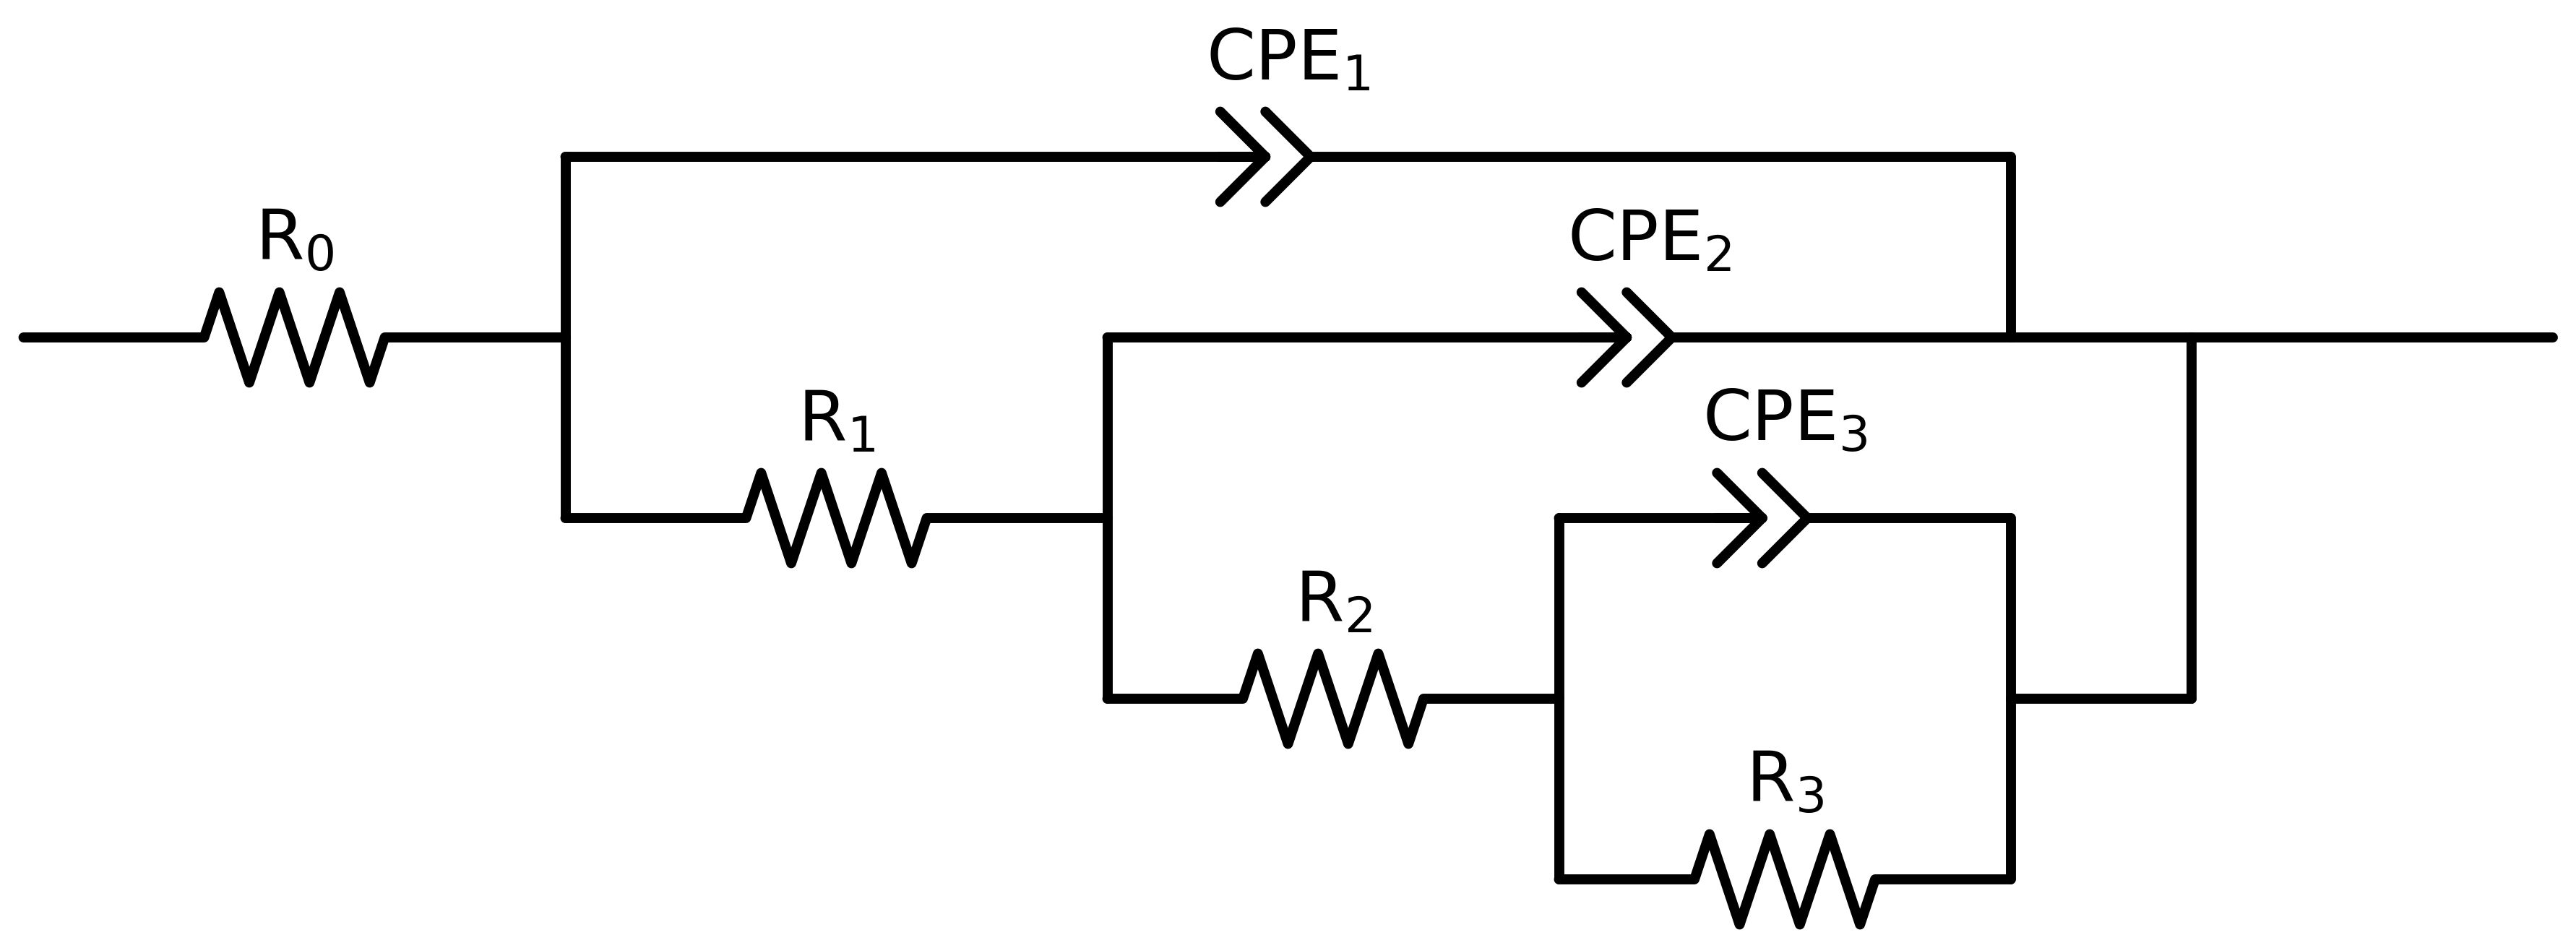
\includegraphics[width=0.45\textwidth]{circuits/3RC.png}
\end{center}

\renewcommand{\arraystretch}{1.6} 
\begin{table}[h!]
    \centering
    \footnotesize
    \begin{tabular}{|l|c|c|c|}
        \hline
        \textbf{Element} & \textbf{Unit} & \textbf{Bounds} & \textbf{Cauvel\_5\_NaVO3\_72H} \\ \hline
        $R_{0}$ & $\Omega$ & $[1.0e+00, 1.0e+03]$ & $5.99e+01 \pm 5.6e-01$ \\ \hline
        $R_{1}$ & $\Omega$ & $[1.0e+00, 1.0e+08]$ & $2.28e+02 \pm 8.0e+01$ \\ \hline
        $R_{2}$ & $\Omega$ & $[1.0e+00, 1.0e+08]$ & $7.23e+03 \pm 3.0e+06$ \\ \hline
        $R_{3}$ & $\Omega$ & $[1.0e+00, 1.0e+08]$ & $8.76e+00 \pm 3.0e+06$ \\ \hline
        $Q_{3}$ & $\Omega$$^{-1}$ sec$^{a}$ & $[1.0e-09, 1.0e-03]$ & $4.11e-08 \pm 2.5e+05$ \\ \hline
        $n_{3}$ & - & $[5.0e-01, 1.0e+00]$ & $7.15e-01 \pm 8.8e+05$ \\ \hline
        $Q_{2}$ & $\Omega$$^{-1}$ sec$^{a}$ & $[1.0e-09, 1.0e-03]$ & $1.33e-04 \pm 3.7e-01$ \\ \hline
        $n_{2}$ & - & $[5.0e-01, 1.0e+00]$ & $7.15e-01 \pm 1.8e-01$ \\ \hline
        $Q_{1}$ & $\Omega$$^{-1}$ sec$^{a}$ & $[1.0e-09, 1.0e-03]$ & $1.51e-04 \pm 4.4e-05$ \\ \hline
        $n_{1}$ & - & $[5.0e-01, 1.0e+00]$ & $6.88e-01 \pm 3.5e-02$ \\ \hline
        \textbf{$\chi^2$} & - & -  & $3.737e-04$ \\ \hline

    \end{tabular}
\end{table}


\newpage
\section*{Analysis Results: 72H}
\begin{center}
    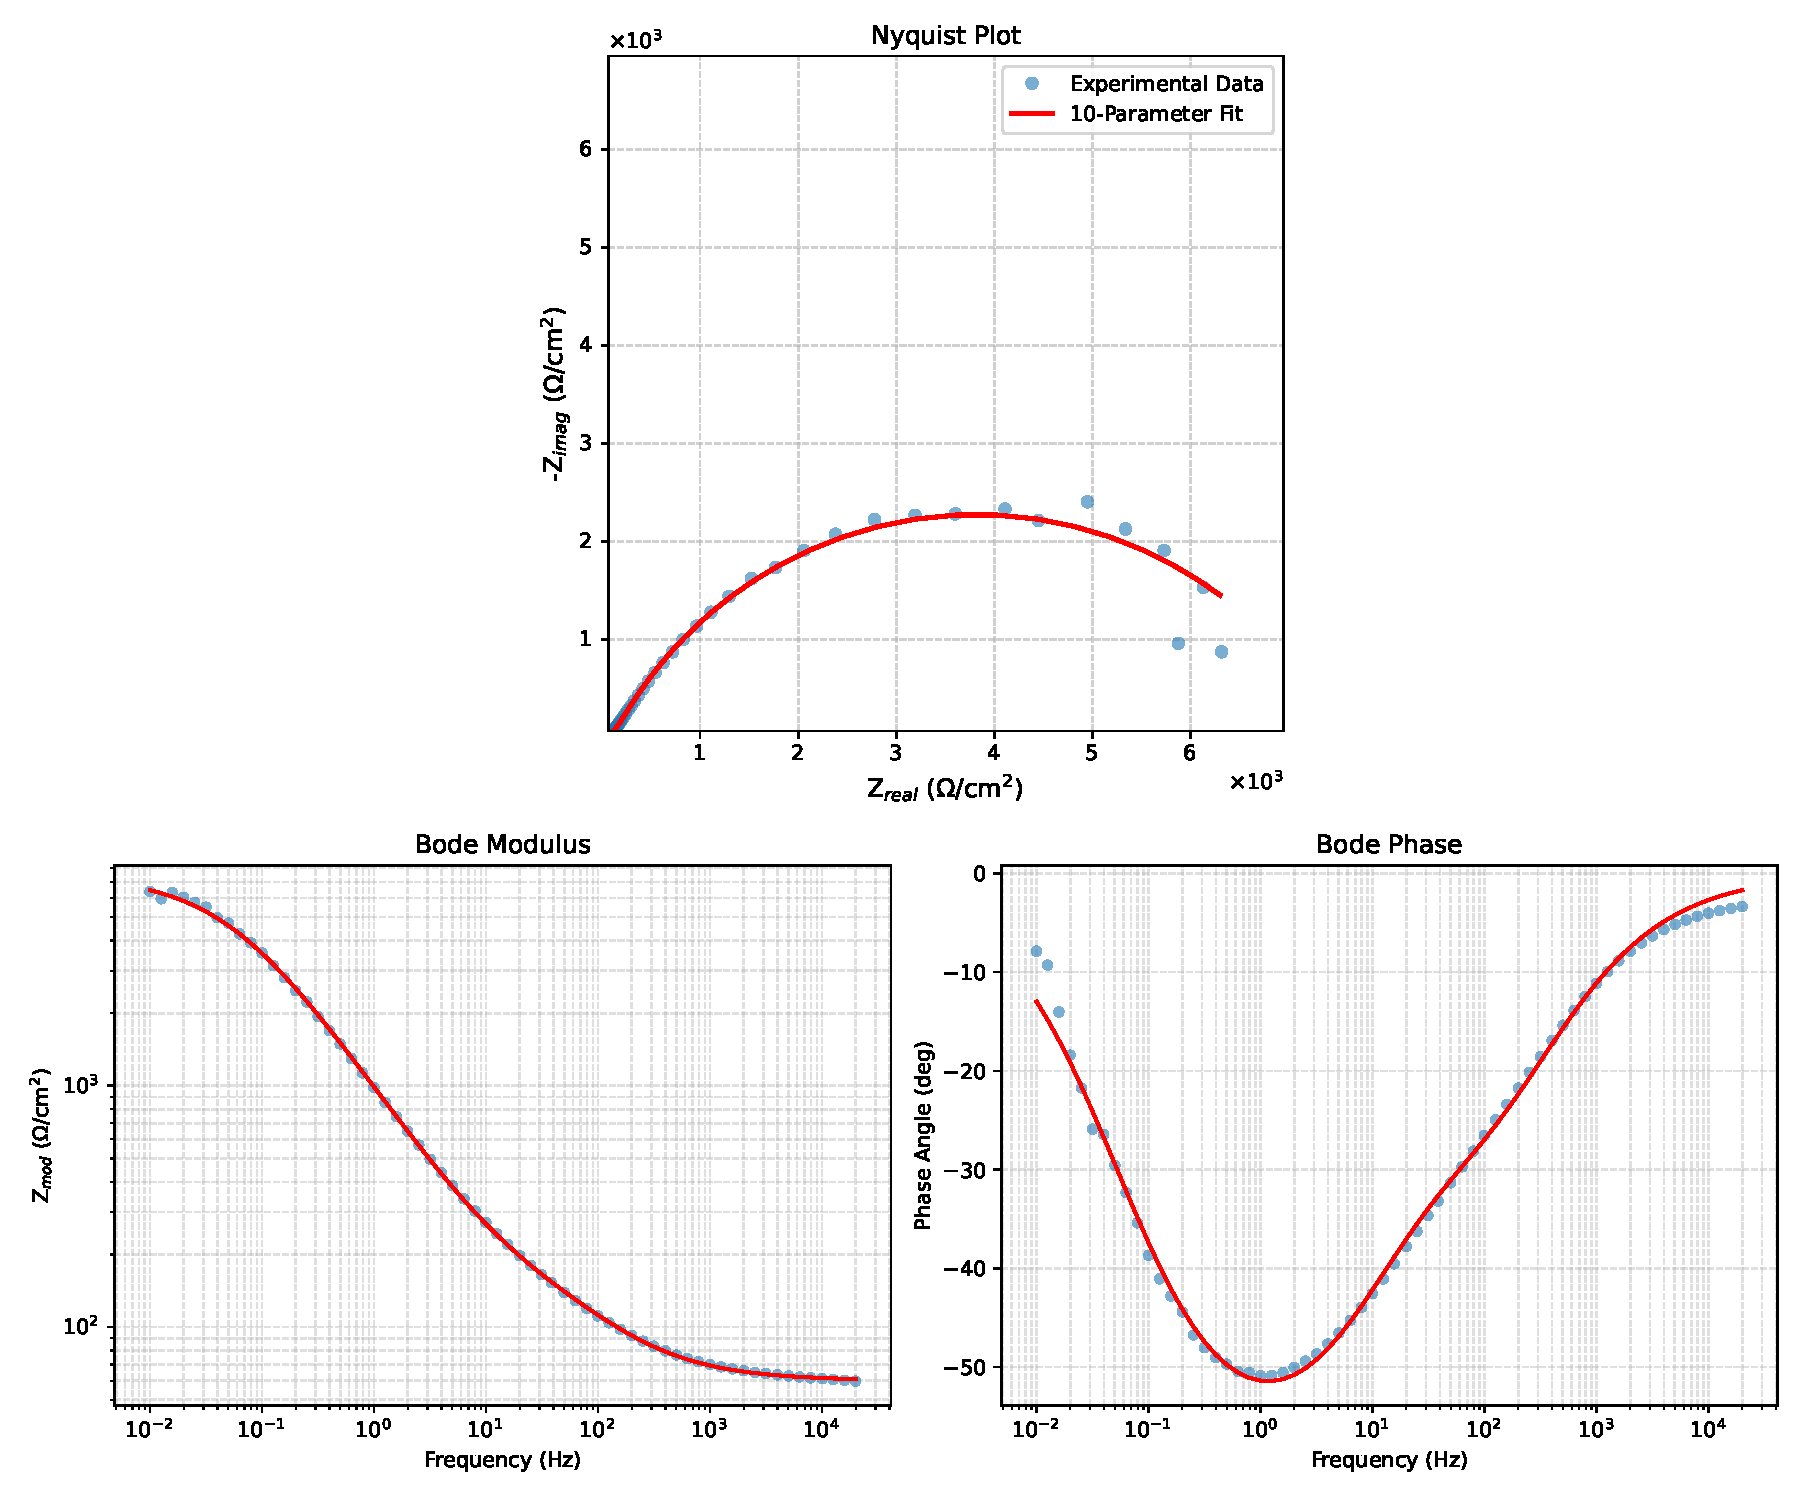
\includegraphics[width=0.7\textwidth]{plots_Cauvel_5_NaVO3_72H_3RC.pdf}
    \captionof{figure}{EIS Fit Results for Cauvel\_5\_NaVO3\_72H}
\end{center}


\end{document}
